\documentclass[12pt]{iptex}
% IDIOMA
% Se necessário, inserir línguas e indicar língua principal (main)
\usepackage[main=brazil,english]{babel}
\usepackage[italic]{mathastext}
\usepackage{siunitx}
\sisetup{
    group-separator={.},
    group-minimum-digits=3,
    output-decimal-marker={,}}

% Alterando nome do TOC (adicionar em outras línguas, se necessário)
\addto\captionsbrazil{%
	\renewcommand{\contentsname}{SUMÁRIO}
	\renewcommand{\refname}{REFERÊNCIAS}
}
\addto\captionsenglish{%
	\renewcommand{\contentsname}{CONTENTS}
	\renewcommand{\refname}{REFERENCES}
}
% BIBLIOGRAFIA
\usepackage[abnt-emphasize=bf,alf]{abntex2cite}
% Para bibliografia ABNT com números
%\usepackage[abnt-emphasize=bf,num]{abntex2cite}
%\citebrackets[]

% Para outros estilos o autor deve definir o \bibliographystyle dentro do documento

% Ajustes adicionais
%\setlist[enumerate]{itemsep=3mm} % espaçamento enumerate
%\setlist[itemize]{itemsep=3mm} % espaçamento itemize

% Início do documento
\begin{document}

% CAPA 
\input{B_Ma_capa.tex}

% Corpo do documento
\section{ÚLTIMOS RELATÓRIOS TÉCNICOS}
\label{sec:ultimos_relatorios}
\begin{itemize}
    \item Relatório Síntese UHMC 2023: Monitoramento sismológico na área do reservatório de Aproveitamento Hidrelétrico de Machadinho, SC/RS, emitido em abril de 2023.
    \item Relatório IPT Nº 205 166 666-1 - “Análise dos registros obtidos entre 01 de dezembro de 2019 e 31 de dezembro de 2021 na rede Sismológica de Itá/Machadinho, RSIM, SC/RS.”, emitido em novembro de 2022.
\end{itemize}

\section{ATIVIDADES REALIZADAS}
\label{sec:atividade}
\begin{itemize}
    \item Encaminhamento do Boletim sísmico nº 25/48-2024, Junho-2023;
    \item Coleta de dados em 01/06/2023 (28/04/2023 a 01/06/2023) e envio dos mesmos para análise no IPT;
    \item Para o período, não houve acesso ao plano de fogo da obra PCH Tupitinga e das pedreiras Engenhos, Kerbermix e PlanaTerra;
    \item Análise preliminar do período que inclui a coleta BCM223118 (31/03/2023 a 28/04/2023) e BCM223152 (28/04/2023 a 01/06/2023); e
    \item Elaboração de gráfico de completeza dos dados, tabela contendo os registros de eventos/detonações detectados.
\end{itemize}

\section{RESULTADOS}
\label{sec:resultados}
Foi detectado um único sismo induzido na região do empreendimento de Machadinho durante o período, na região do remanso do reservatório, com magnitude -0.5 MLv, evento pequeno, em 2023-05-21 21:54:53 (UTC). Não há relatos de eventos que tenham sido sentidos pela população local.

Foram detectados 4 (quatro) desmontes durante o período, sendo o de maior magnitude em 2023-05-19 16:05:43 (UTC) com magnitude 2.0 MLv. Três dos desmontes ocorreram longe da região do reservatório (incluindo o de maior magnitude) e um próximo à cidade de Campos Novos – SC.

Não foram detectados sismos naturais regionais e/ou telessismos no território brasileiro durante o período englobado por este boletim na estação BCM2.

Os parâmetros sísmicos dos eventos detectados são detalhados na Tabela 1. O gráfico de completeza dos dados para a estação BCM2 no mês de maio/2023 é mostrado na Figura 1.

O funcionamento da estação BCM2 foi adequado no mês de maio/2023. A estação MC9 se encontra avariada, conforme detalhado no boletim sísmico Nº 38/48-2021 Jul.20. O digitalizador da estação se encontra na sede do IPT em São Paulo. Recomendações para resumir o funcionamento da estação já foram repassadas pelo IPT à ENGIE, e a empresa já iniciou o processo de aquisição de novos equipamentos.

\section{CONSIDERAÇÕES}
\label{sec:consideracoes}
Continuam válidas as considerações e orientações anteriores a respeito das medidas a serem tomadas em caso ocorrência de um sismo local sentido pela população, i.e., coletar os relatos da população local através de questionários macrossísmicos, contactar a defesa civil para avaliar possíveis danos em estruturas e fornecer orientações e informações à população.

A estação MC9, conforme discutido em boletim anterior, não está operando no momento. Recomendações para resumir o funcionamento da estação já foram repassadas pelo IPT à ENGIE, e a empresa já iniciou o processo de aquisição de novos equipamentos.

%\datahoje{São Paulo, 25 de agosto de 2023}

INSERIR ASSINATURA!
INSERIR ASSINATURA!
INSERIR ASSINATURA!
INSERIR ASSINATURA!
INSERIR ASSINATURA!
INSERIR ASSINATURA!



\section{COMPLETUDE DOS DADOS}

\label{fig:completude}
\begin{figure}[htb!]
    \centering
	\captionsetup{justification=raggedright, singlelinecheck=false, width=1\textwidth}
    \caption{Gráfico de completude dos dados para o mês de MÊS para estação ESTAÇÃO.}
    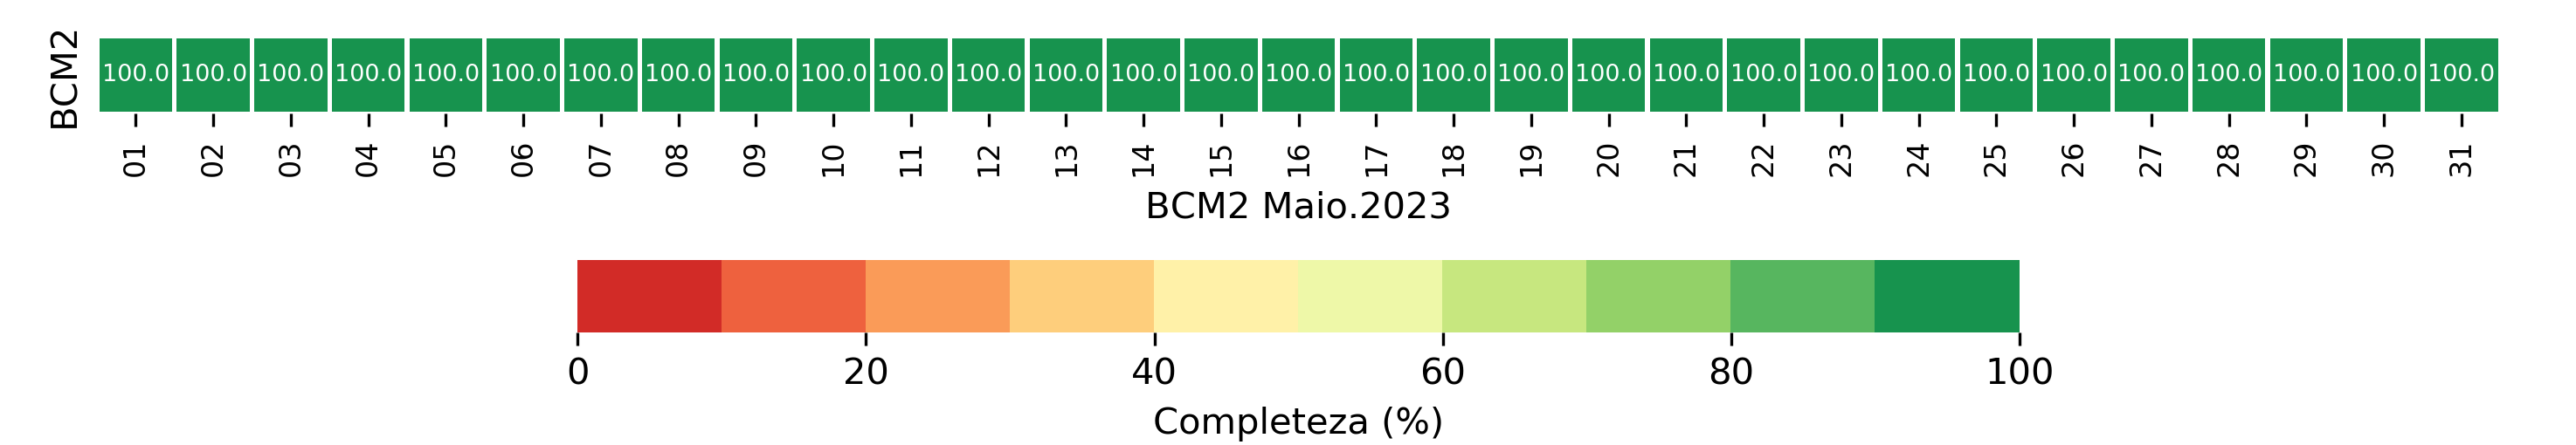
\includegraphics[width=1.0\textwidth]{../figuras/completude.png} % Substitua pelo nome da imagem e ajuste o tamanho
    \caption*{Fonte:IPT}
	\label{fig:completude}
\end{figure}



\section{TABELA DE EVENTOS}
\label{sec:tabelas}
\begin{center}
\setcaptionmargin{1cm}
\scriptsize
\begin{longtable}{lcccccccc}
\caption[Exemplo de tabela.]{Dados de Terremotos}\\
\hline \hline\\[-2ex]
\multicolumn{1}{c}{ID} &
\multicolumn{1}{c}{Hora de Origem (UTC)} &
\multicolumn{1}{c}{Longitude} &
\multicolumn{1}{c}{Latitude} &
\multicolumn{1}{c}{UTM X} &
\multicolumn{1}{c}{UTM Y} &
\multicolumn{1}{c}{MLv} &
\multicolumn{1}{c}{Energia} &
\multicolumn{1}{c}{Cat} 

\\[0.5ex] \hline
\\[-1.8ex]

\multicolumn{1}{c}{} & 
\multicolumn{1}{c}{} & 
\multicolumn{1}{c}(\textdegree\hspace{0.25em}) & 
\multicolumn{1}{c}(\textdegree\hspace{0.25em}) & 
\multicolumn{1}{c}{(m)} & 
\multicolumn{1}{c}{(m)} & 
\multicolumn{1}{c}{} & 
\multicolumn{1}{c}{(J)} & 
\multicolumn{1}{c}{} 

\\[0.5ex] \hline
\\[-1.8ex]


\endfirsthead

\multicolumn{9}{c}{\footnotesize{{\slshape{{\tablename} \table{}}} - Continuação}}\\[0.5ex]

\hline \hline\\[-2ex]

\multicolumn{1}{c}{ID} &
\multicolumn{1}{c}{Hora de Origem (UTC)} &
\multicolumn{1}{c}{Longitude} &
\multicolumn{1}{c}{Latitude} &
\multicolumn{1}{c}{UTM X} &
\multicolumn{1}{c}{UTM Y} &
\multicolumn{1}{c}{MLv} &
\multicolumn{1}{c}{Energia} &
\multicolumn{1}{c}{Cat}

\\[0.5ex] \hline
\\[-1.8ex]

\multicolumn{1}{c}{} & 
\multicolumn{1}{c}{} & 
\multicolumn{1}{c}(\textdegree\hspace{0.25em}) & 
\multicolumn{1}{c}(\textdegree\hspace{0.25em}) & 
\multicolumn{1}{c}{(m)} & 
\multicolumn{1}{c}{(m)} & 
\multicolumn{1}{c}{} & 
\multicolumn{1}{c}{(J)} & 
\multicolumn{1}{c}{} 

\\[0.5ex] \hline
\\[-1.8ex]


\endhead

\multicolumn{3}{l}{\footnotesize{Continua na próxima página\ldots}}}\\
\endfoot
\hline

\endlastfoot
IT\_20230630\_070654 & 2023-06-30T07:06:54 & -52,1236 & -27,2447 & 388756 & 6985959 & -0,5 & \num[round-precision=3,round-mode=figures,scientific-notation=true]{80.6926} & I \\
IT\_20230623\_033615 & 2023-06-23T03:36:15 & -52,0635 & -27,3083 & 394770 & 6978969 & -0,5 & \num[round-precision=3,round-mode=figures,scientific-notation=true]{82.288} & I \\
IT\_20230622\_193901 & 2023-06-22T19:39:01 & -52,2639 & -27,2941 & 374921 & 6980353 & -0,6 & \num[round-precision=3,round-mode=figures,scientific-notation=true]{69.5138} & I \\
IT\_20230622\_190347 & 2023-06-22T19:03:47 & -52,4587 & -27,6399 & 356096 & 6941839 & 0,9 & \num[round-precision=3,round-mode=figures,scientific-notation=true]{34691.7} & Q \\
IT\_20230621\_045910 & 2023-06-21T04:59:10 & -52,3299 & -27,3139 & 368411 & 6978098 & -0,7 & \num[round-precision=3,round-mode=figures,scientific-notation=true]{33.2441} & I \\
IT\_20230619\_163424 & 2023-06-19T16:34:24 & -53,0940 & -28,4311 & 294913 & 6853250 & 1,3 & \num[round-precision=3,round-mode=figures,scientific-notation=true]{262839} & Q \\
gfz2023lsea & 2023-06-16T11:22:00 & -47,4000 & -24,5000 & 256798 & 7288301 & 5,2 & \num[round-precision=3,round-mode=figures,scientific-notation=true]{4.34826e+12} & E \\
IT\_20230613\_091716 & 2023-06-13T09:17:16 & -52,3448 & -27,3051 & 366930 & 6979050 & 0,3 & \num[round-precision=3,round-mode=figures,scientific-notation=true]{2568.54} & I \\
IT\_20230611\_190546 & 2023-06-11T19:05:46 & -52,1223 & -27,2430 & 388886 & 6986149 & -0,1 & \num[round-precision=3,round-mode=figures,scientific-notation=true]{625.703} & I \\
IT\_20230608\_063905 & 2023-06-08T06:39:05 & -52,1233 & -27,2441 & 388790 & 6986031 & -0,6 & \num[round-precision=3,round-mode=figures,scientific-notation=true]{48.8092} & I \\
IT\_20230606\_173127 & 2023-06-06T17:31:27 & -52,5289 & -27,4790 & 348949 & 6959577 & 1,2 & \num[round-precision=3,round-mode=figures,scientific-notation=true]{125331} & Q \\
IT\_20230606\_003357 & 2023-06-06T00:33:57 & -52,1642 & -27,2142 & 384706 & 6989301 & -0,9 & \num[round-precision=3,round-mode=figures,scientific-notation=true]{17.2632} & I \\
IT\_20230605\_203509 & 2023-06-05T20:35:09 & -51,7175 & -27,3387 & 429030 & 6975842 & 0,8 & \num[round-precision=3,round-mode=figures,scientific-notation=true]{29450.1} & Q \\
IT\_20230601\_195756 & 2023-06-01T19:57:56 & -52,0606 & -27,2107 & 394964 & 6989781 & 0,9 & \num[round-precision=3,round-mode=figures,scientific-notation=true]{38000.7} & Q \\
IT\_20230601\_055456 & 2023-06-01T05:54:56 & -52,1247 & -27,2432 & 388648 & 6986122 & -0,9 & \num[round-precision=3,round-mode=figures,scientific-notation=true]{18.0537} & I \\
IT\_20230630\_070654 & 2023-06-30T07:06:54 & -52,1236 & -27,2447 & 388756 & 6985959 & -0,5 & \num[round-precision=3,round-mode=figures,scientific-notation=true]{80.6926} & I \\
IT\_20230623\_033615 & 2023-06-23T03:36:15 & -52,0635 & -27,3083 & 394770 & 6978969 & -0,5 & \num[round-precision=3,round-mode=figures,scientific-notation=true]{82.288} & I \\
IT\_20230622\_193901 & 2023-06-22T19:39:01 & -52,2639 & -27,2941 & 374921 & 6980353 & -0,6 & \num[round-precision=3,round-mode=figures,scientific-notation=true]{69.5138} & I \\
IT\_20230622\_190347 & 2023-06-22T19:03:47 & -52,4587 & -27,6399 & 356096 & 6941839 & 0,9 & \num[round-precision=3,round-mode=figures,scientific-notation=true]{34691.7} & Q \\
IT\_20230621\_045910 & 2023-06-21T04:59:10 & -52,3299 & -27,3139 & 368411 & 6978098 & -0,7 & \num[round-precision=3,round-mode=figures,scientific-notation=true]{33.2441} & I \\
IT\_20230619\_163424 & 2023-06-19T16:34:24 & -53,0940 & -28,4311 & 294913 & 6853250 & 1,3 & \num[round-precision=3,round-mode=figures,scientific-notation=true]{262839} & Q \\
gfz2023lsea & 2023-06-16T11:22:00 & -47,4000 & -24,5000 & 256798 & 7288301 & 5,2 & \num[round-precision=3,round-mode=figures,scientific-notation=true]{4.34826e+12} & E \\
IT\_20230613\_091716 & 2023-06-13T09:17:16 & -52,3448 & -27,3051 & 366930 & 6979050 & 0,3 & \num[round-precision=3,round-mode=figures,scientific-notation=true]{2568.54} & I \\
IT\_20230611\_190546 & 2023-06-11T19:05:46 & -52,1223 & -27,2430 & 388886 & 6986149 & -0,1 & \num[round-precision=3,round-mode=figures,scientific-notation=true]{625.703} & I \\
IT\_20230608\_063905 & 2023-06-08T06:39:05 & -52,1233 & -27,2441 & 388790 & 6986031 & -0,6 & \num[round-precision=3,round-mode=figures,scientific-notation=true]{48.8092} & I \\
IT\_20230606\_173127 & 2023-06-06T17:31:27 & -52,5289 & -27,4790 & 348949 & 6959577 & 1,2 & \num[round-precision=3,round-mode=figures,scientific-notation=true]{125331} & Q \\
IT\_20230606\_003357 & 2023-06-06T00:33:57 & -52,1642 & -27,2142 & 384706 & 6989301 & -0,9 & \num[round-precision=3,round-mode=figures,scientific-notation=true]{17.2632} & I \\
IT\_20230605\_203509 & 2023-06-05T20:35:09 & -51,7175 & -27,3387 & 429030 & 6975842 & 0,8 & \num[round-precision=3,round-mode=figures,scientific-notation=true]{29450.1} & Q \\
IT\_20230601\_195756 & 2023-06-01T19:57:56 & -52,0606 & -27,2107 & 394964 & 6989781 & 0,9 & \num[round-precision=3,round-mode=figures,scientific-notation=true]{38000.7} & Q \\
IT\_20230601\_055456 & 2023-06-01T05:54:56 & -52,1247 & -27,2432 & 388648 & 6986122 & -0,9 & \num[round-precision=3,round-mode=figures,scientific-notation=true]{18.0537} & I \\
IT\_20230630\_070654 & 2023-06-30T07:06:54 & -52,1236 & -27,2447 & 388756 & 6985959 & -0,5 & \num[round-precision=3,round-mode=figures,scientific-notation=true]{80.6926} & I \\
IT\_20230623\_033615 & 2023-06-23T03:36:15 & -52,0635 & -27,3083 & 394770 & 6978969 & -0,5 & \num[round-precision=3,round-mode=figures,scientific-notation=true]{82.288} & I \\
IT\_20230622\_193901 & 2023-06-22T19:39:01 & -52,2639 & -27,2941 & 374921 & 6980353 & -0,6 & \num[round-precision=3,round-mode=figures,scientific-notation=true]{69.5138} & I \\
IT\_20230622\_190347 & 2023-06-22T19:03:47 & -52,4587 & -27,6399 & 356096 & 6941839 & 0,9 & \num[round-precision=3,round-mode=figures,scientific-notation=true]{34691.7} & Q \\
IT\_20230621\_045910 & 2023-06-21T04:59:10 & -52,3299 & -27,3139 & 368411 & 6978098 & -0,7 & \num[round-precision=3,round-mode=figures,scientific-notation=true]{33.2441} & I \\
IT\_20230619\_163424 & 2023-06-19T16:34:24 & -53,0940 & -28,4311 & 294913 & 6853250 & 1,3 & \num[round-precision=3,round-mode=figures,scientific-notation=true]{262839} & Q \\
gfz2023lsea & 2023-06-16T11:22:00 & -47,4000 & -24,5000 & 256798 & 7288301 & 5,2 & \num[round-precision=3,round-mode=figures,scientific-notation=true]{4.34826e+12} & E \\
IT\_20230613\_091716 & 2023-06-13T09:17:16 & -52,3448 & -27,3051 & 366930 & 6979050 & 0,3 & \num[round-precision=3,round-mode=figures,scientific-notation=true]{2568.54} & I \\
IT\_20230611\_190546 & 2023-06-11T19:05:46 & -52,1223 & -27,2430 & 388886 & 6986149 & -0,1 & \num[round-precision=3,round-mode=figures,scientific-notation=true]{625.703} & I \\
IT\_20230608\_063905 & 2023-06-08T06:39:05 & -52,1233 & -27,2441 & 388790 & 6986031 & -0,6 & \num[round-precision=3,round-mode=figures,scientific-notation=true]{48.8092} & I \\
IT\_20230606\_173127 & 2023-06-06T17:31:27 & -52,5289 & -27,4790 & 348949 & 6959577 & 1,2 & \num[round-precision=3,round-mode=figures,scientific-notation=true]{125331} & Q \\
IT\_20230606\_003357 & 2023-06-06T00:33:57 & -52,1642 & -27,2142 & 384706 & 6989301 & -0,9 & \num[round-precision=3,round-mode=figures,scientific-notation=true]{17.2632} & I \\
IT\_20230605\_203509 & 2023-06-05T20:35:09 & -51,7175 & -27,3387 & 429030 & 6975842 & 0,8 & \num[round-precision=3,round-mode=figures,scientific-notation=true]{29450.1} & Q \\
IT\_20230601\_195756 & 2023-06-01T19:57:56 & -52,0606 & -27,2107 & 394964 & 6989781 & 0,9 & \num[round-precision=3,round-mode=figures,scientific-notation=true]{38000.7} & Q \\
IT\_20230601\_055456 & 2023-06-01T05:54:56 & -52,1247 & -27,2432 & 388648 & 6986122 & -0,9 & \num[round-precision=3,round-mode=figures,scientific-notation=true]{18.0537} & I \\
IT\_20230630\_070654 & 2023-06-30T07:06:54 & -52,1236 & -27,2447 & 388756 & 6985959 & -0,5 & \num[round-precision=3,round-mode=figures,scientific-notation=true]{80.6926} & I \\
IT\_20230623\_033615 & 2023-06-23T03:36:15 & -52,0635 & -27,3083 & 394770 & 6978969 & -0,5 & \num[round-precision=3,round-mode=figures,scientific-notation=true]{82.288} & I \\
IT\_20230622\_193901 & 2023-06-22T19:39:01 & -52,2639 & -27,2941 & 374921 & 6980353 & -0,6 & \num[round-precision=3,round-mode=figures,scientific-notation=true]{69.5138} & I \\
IT\_20230622\_190347 & 2023-06-22T19:03:47 & -52,4587 & -27,6399 & 356096 & 6941839 & 0,9 & \num[round-precision=3,round-mode=figures,scientific-notation=true]{34691.7} & Q \\
IT\_20230621\_045910 & 2023-06-21T04:59:10 & -52,3299 & -27,3139 & 368411 & 6978098 & -0,7 & \num[round-precision=3,round-mode=figures,scientific-notation=true]{33.2441} & I \\
IT\_20230619\_163424 & 2023-06-19T16:34:24 & -53,0940 & -28,4311 & 294913 & 6853250 & 1,3 & \num[round-precision=3,round-mode=figures,scientific-notation=true]{262839} & Q \\
gfz2023lsea & 2023-06-16T11:22:00 & -47,4000 & -24,5000 & 256798 & 7288301 & 5,2 & \num[round-precision=3,round-mode=figures,scientific-notation=true]{4.34826e+12} & E \\
IT\_20230613\_091716 & 2023-06-13T09:17:16 & -52,3448 & -27,3051 & 366930 & 6979050 & 0,3 & \num[round-precision=3,round-mode=figures,scientific-notation=true]{2568.54} & I \\
IT\_20230611\_190546 & 2023-06-11T19:05:46 & -52,1223 & -27,2430 & 388886 & 6986149 & -0,1 & \num[round-precision=3,round-mode=figures,scientific-notation=true]{625.703} & I \\
IT\_20230608\_063905 & 2023-06-08T06:39:05 & -52,1233 & -27,2441 & 388790 & 6986031 & -0,6 & \num[round-precision=3,round-mode=figures,scientific-notation=true]{48.8092} & I \\
IT\_20230606\_173127 & 2023-06-06T17:31:27 & -52,5289 & -27,4790 & 348949 & 6959577 & 1,2 & \num[round-precision=3,round-mode=figures,scientific-notation=true]{125331} & Q \\
IT\_20230606\_003357 & 2023-06-06T00:33:57 & -52,1642 & -27,2142 & 384706 & 6989301 & -0,9 & \num[round-precision=3,round-mode=figures,scientific-notation=true]{17.2632} & I \\
IT\_20230605\_203509 & 2023-06-05T20:35:09 & -51,7175 & -27,3387 & 429030 & 6975842 & 0,8 & \num[round-precision=3,round-mode=figures,scientific-notation=true]{29450.1} & Q \\
IT\_20230601\_195756 & 2023-06-01T19:57:56 & -52,0606 & -27,2107 & 394964 & 6989781 & 0,9 & \num[round-precision=3,round-mode=figures,scientific-notation=true]{38000.7} & Q \\
IT\_20230601\_055456 & 2023-06-01T05:54:56 & -52,1247 & -27,2432 & 388648 & 6986122 & -0,9 & \num[round-precision=3,round-mode=figures,scientific-notation=true]{18.0537} & I \\



\label{tab:dados_terremoto}
%\caption*{Fonte:IPT.}
\end{longtable}
\end{center}


\section{MAPA DE EVENTOS}
\label{sec:mapa}
\begin{figure}[ht]
    \centering
	\captionsetup{justification=raggedright, singlelinecheck=false, width=1\textwidth}
    \caption{Mapa de eventos.}
    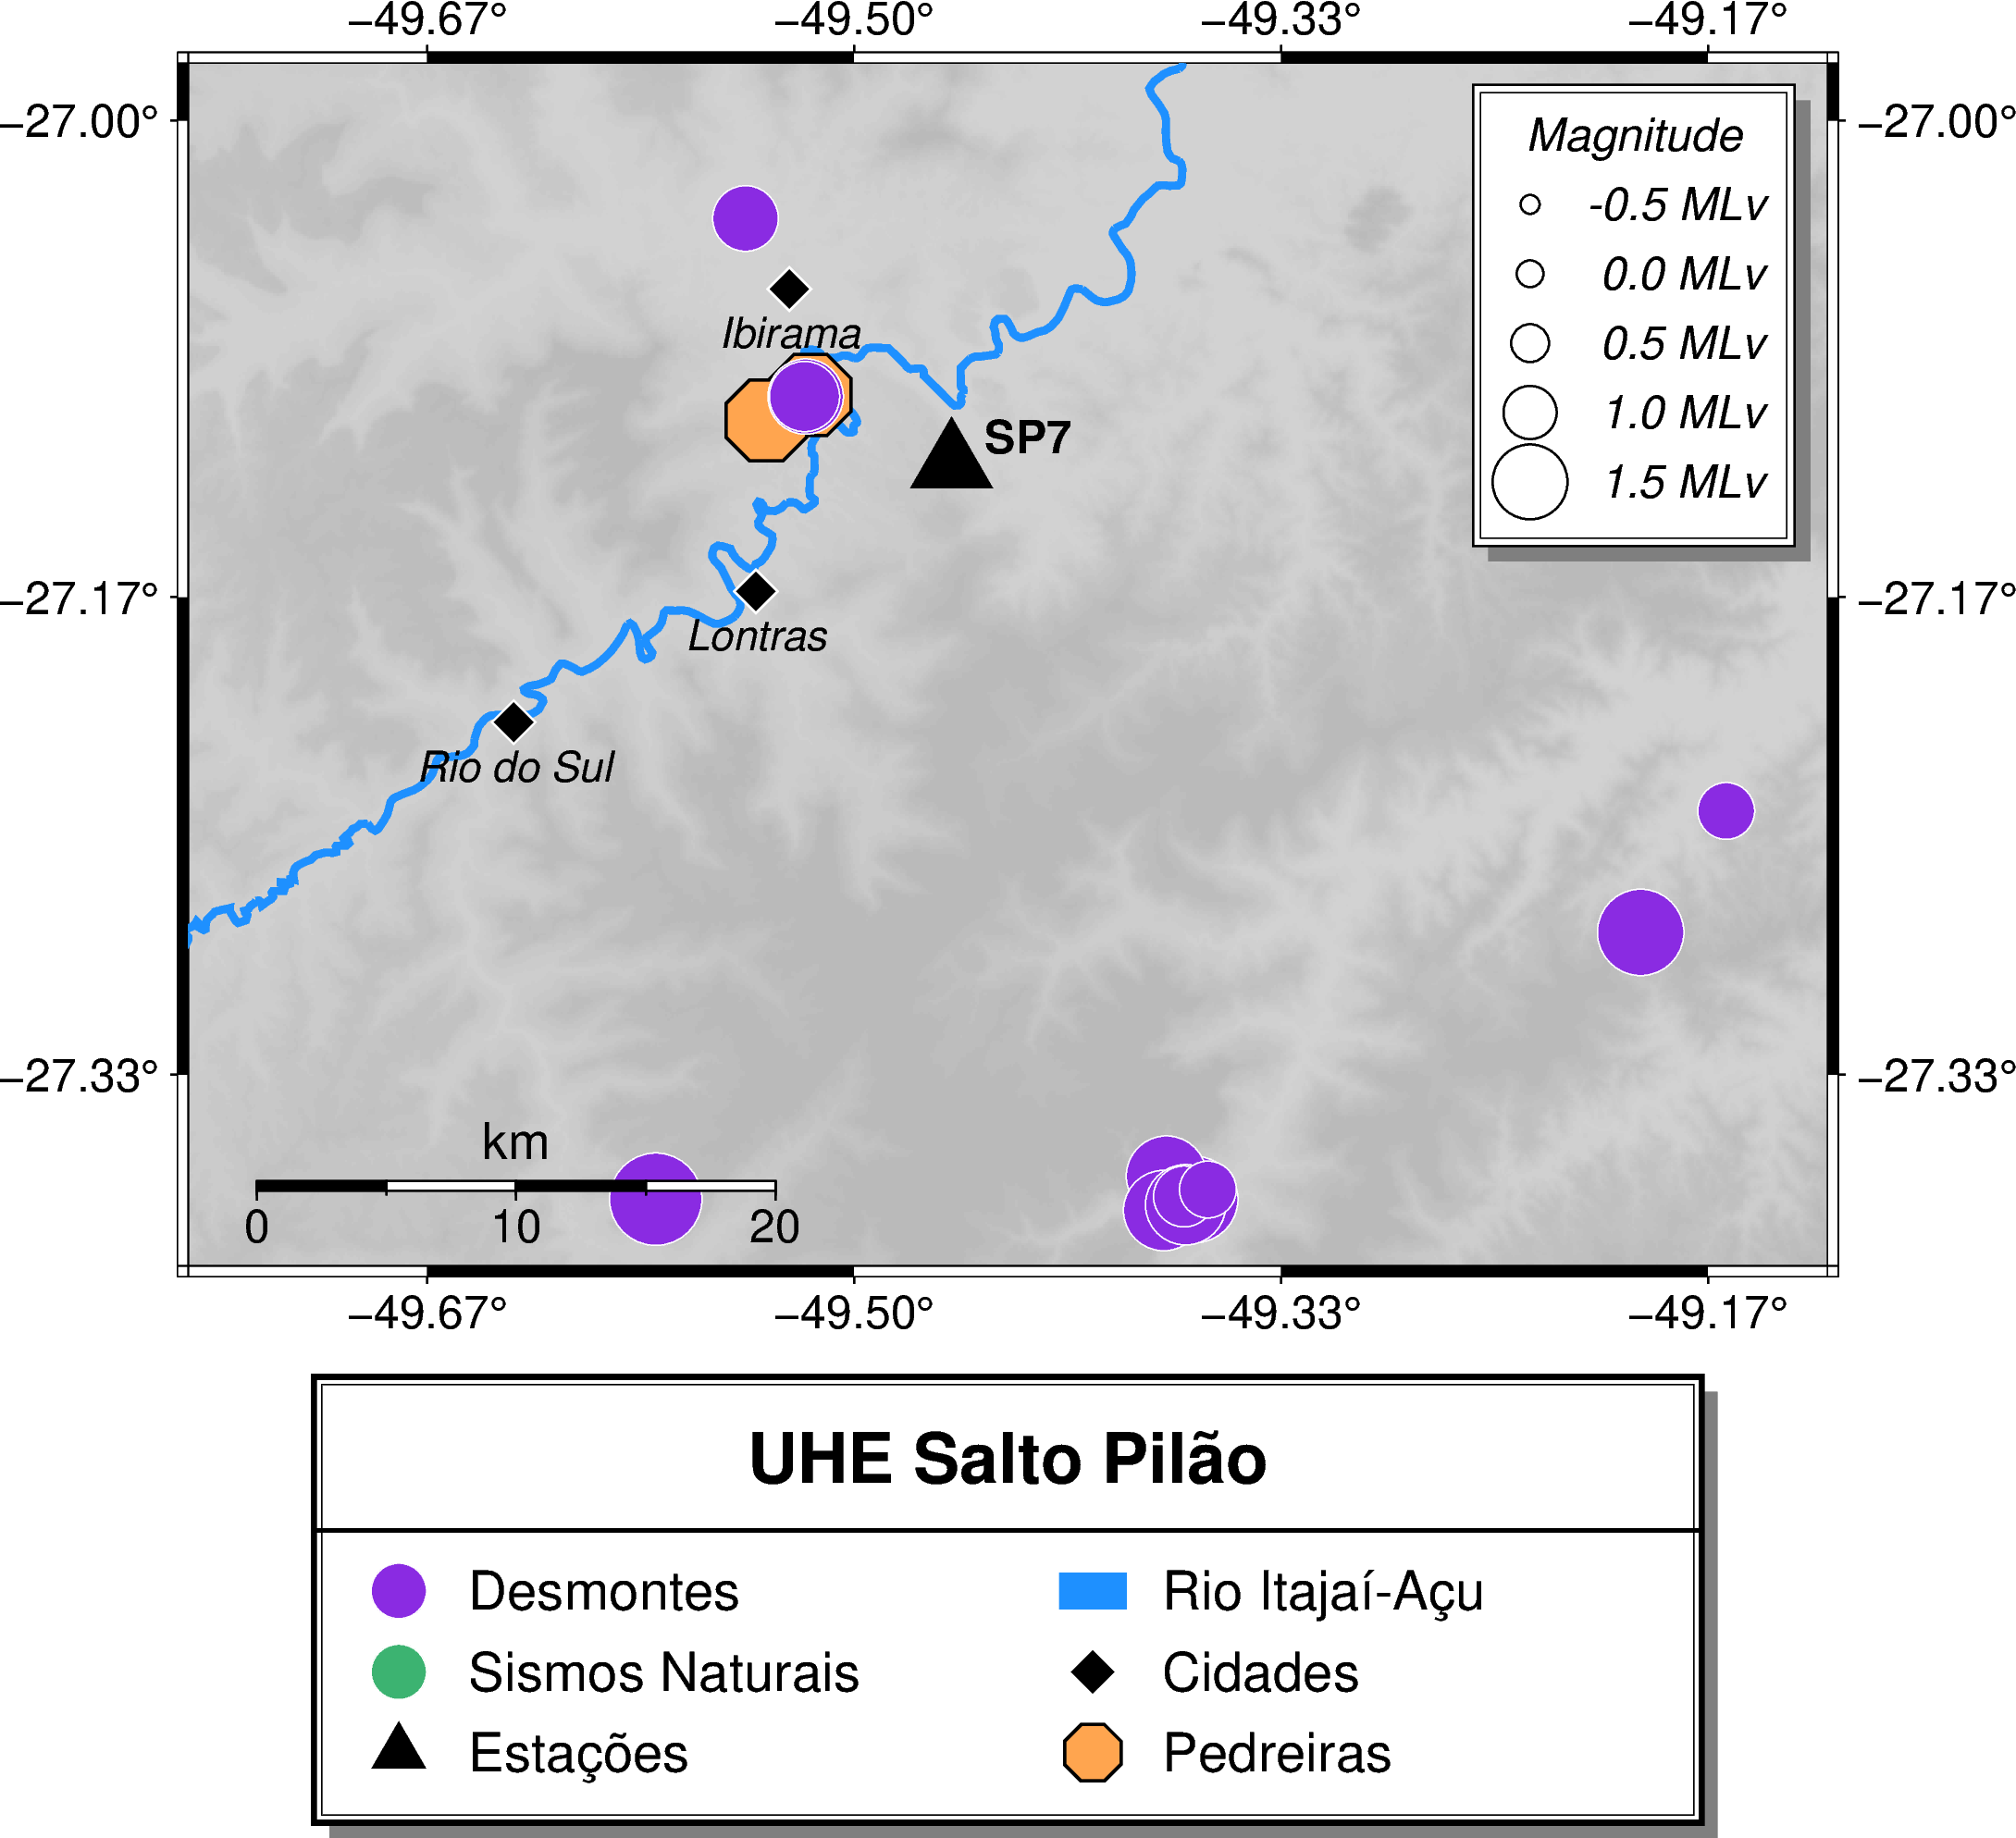
\includegraphics[width=1.0\textwidth]{figuras/mapaevents.png} % Substitua pelo nome do arquivo de imagem e ajuste o tamanho
    \caption*{Fonte:IPT}
\end{figure}



\section{REFERÊNCIAS BIBLIOGRÁFICAS}
% Bibliografia
%\renewcommand{\refname}{REFERÊNCIAS}
%\%addcontentsline{toc}{section}{REFERÊNCIAS}
%\bibliography{ref}


\end{document}
